\documentclass[11pt]{amsbook}

\usepackage{../HBSuerDemir}	% ------------------------


\begin{document}

% ++++++++++++++++++++++++++++++++++++++
\hPage{b2p1/205}
% ++++++++++++++++++++++++++++++++++++++

\noindent intersecting a given curve $\Gamma$ (or remaining tangent to a given surface $\Sigma$).

\begin{defn}
Equation of a surface of revolution: The equation of the surface defined by $\Delta \cong \text{z-axis}$,
\[
\Gamma: x = f(t), \quad y=g(t), \quad z=h(t)
\]
\end{defn} 

\begin{figure}[htbp]
        \centering
            \centering
            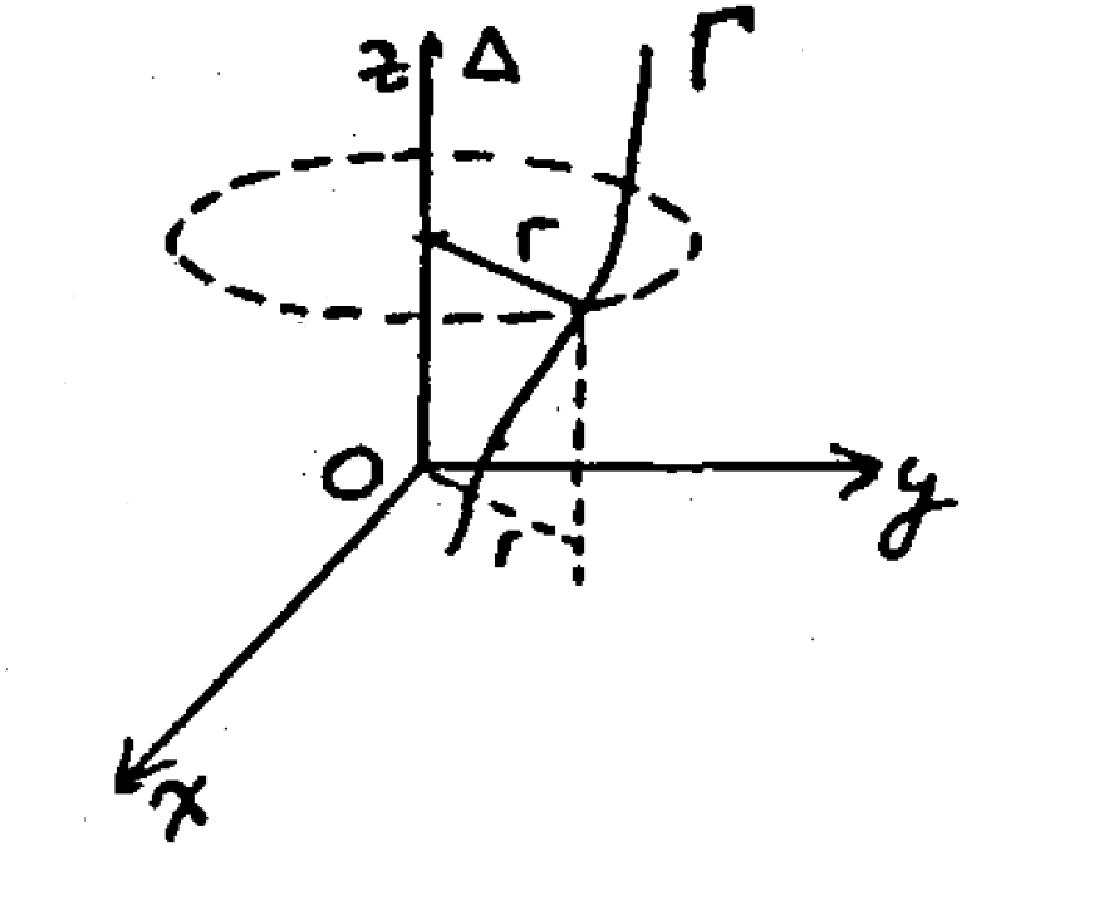
\includegraphics[width=0.25\textwidth]{images/b2p1-205-fig01.pdf}
	        \caption{Surface of revolution}
        	\label{fig:SurfaceOfRevolution}
    \end{figure}   

\begin{hSolution}
The equation of the ``parallel" circle through $P(f(t))$, $g(t)$, $h(t)$ being
\[    
x^2+y^2=r^2, \quad z=h(t)
\]
where $r^2=f^2(t)+g^2(t)$, we have the parametric equation
\[    
S:\quad x^2+y^2 = f^2(t)+g^2(t),\quad z=h(t)
\]
Eliminating $t$ between the two relations, one gets
\[    
S:\quad F(x,y,z) = 0
\]
\end{hSolution}

\begin{exmp}
Find the cartesian equation of the surface generated by revolving
\[    
\Gamma:\quad x=t,\quad y=t-2, \quad x=t^2
\]
about z-axis.
\end{exmp}

\begin{hSolution}
\begin{align*}
& &&x^2+y^2=r^2, &&z=t^2, \quad \text{with } r^2=t^2+(t-2)^2\\
&\Rightarrow \quad && x^2+y^2=t^2+(t-2)^2, &&z=t^2\\
&\Rightarrow \quad && x^2+y^2=2t^2-4t+4,\quad&& z=t^2\\
&\Rightarrow \quad && x^2+y^2=2z-4t+4, &&z=t^2\\
&\Rightarrow \quad && (x^2+y^2-2z-4)^2 = 16z.\\
\end{align*}
\end{hSolution}

% =======================================================
\end{document}